\chapter{Application}

    Nous avons exploité une base de données de \~80.000 photos géolocalisées extraites de Flickr dans le cadre d'une découverte
    non-assistée de points d'intêrets, avec catégorisation et filtrage de ces derniers. (comme c'est le cas sur Google Maps, par exemple)

    Pour cela, nous nous sommes d'abord familiarisés avec les données, décidé des données à garder, nettoyé le document (csv) contenant ces dernières et expérimenté quelques méthodes de clustering avec Knime.

    Nous sommes ensuite passé en production avec un stack Python~: pandas pour le traitement et la sélection des données, numpy et scikits-learn pour le clustering et flask pour servir notre application web.

    Nous discuterons toutes ces étapes avec plus de détails dans les sections à suivre, mais nous vous invitons vivement à d'abord
    tester \href{http://188.226.171.22:5000}{\textbf{notre application web}}. Si elle n'est pas disponible (à cause du firewall de
    l'INSA, par exemple), vous pouvez aussi voir \href{http://www.youtube.com/watch?v=DjlNwlbRyMo}{\textbf{ce court screencast}} faisant la démonstration de ses principales fonctionnalités.

    Voici aussi quelques screenshots de l'application~:

    \begin{figure}[H]
        \centering
        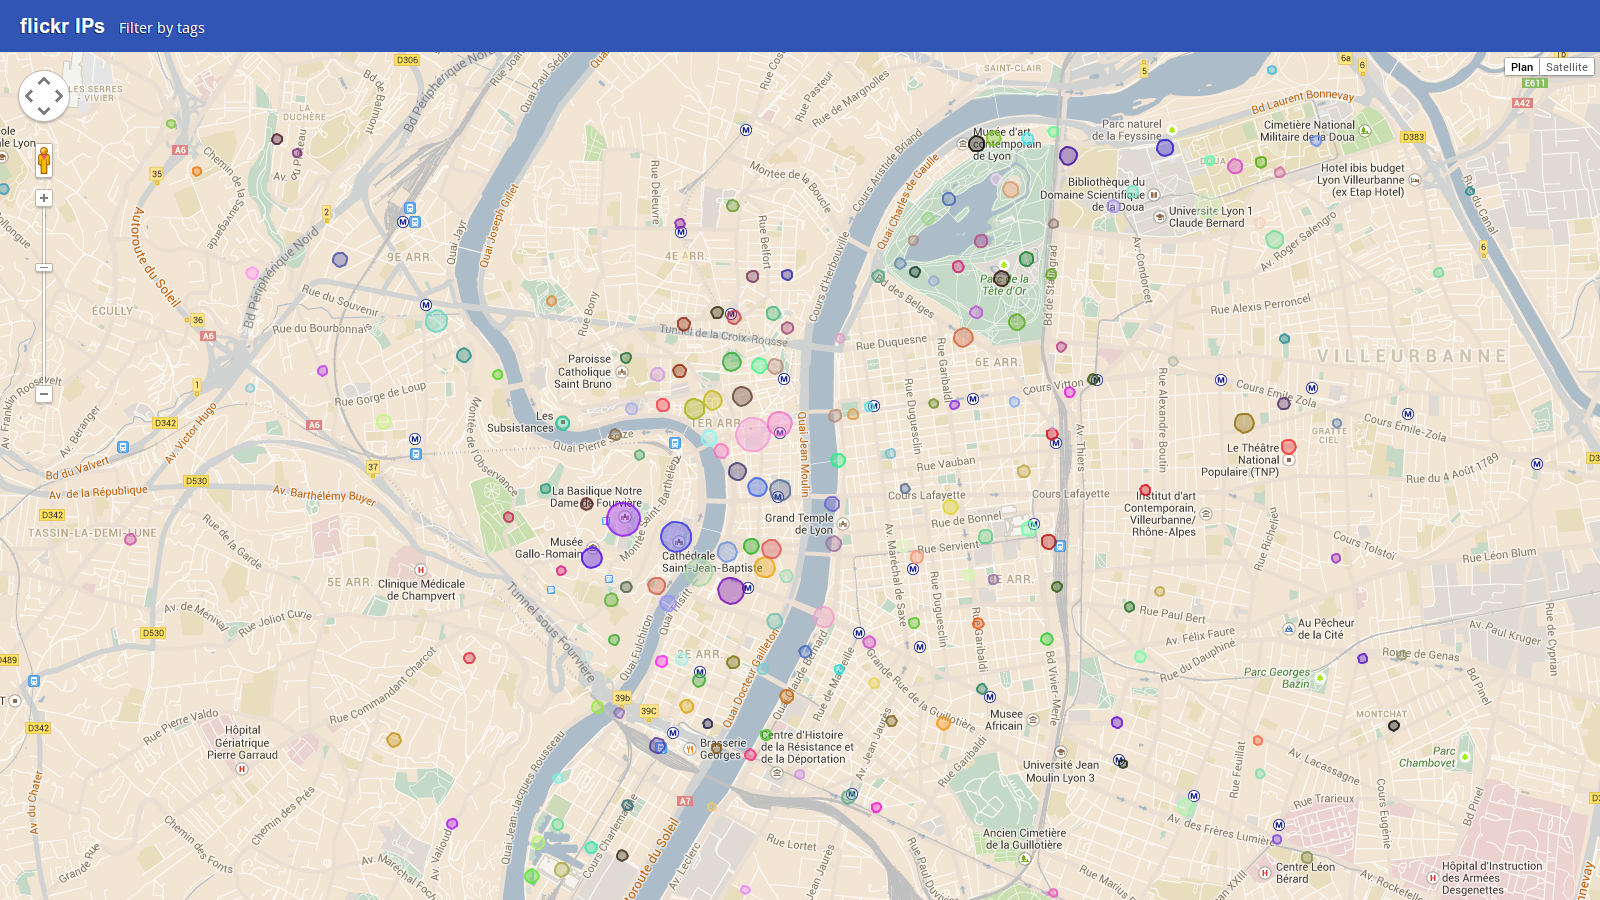
\includegraphics[scale=0.25]{../screenshots/ui-global.png}
        \caption{Interface globale de l'application}
        \label{diagram:ui-global}
    \end{figure}


    \begin{figure}[H]
        \centering
        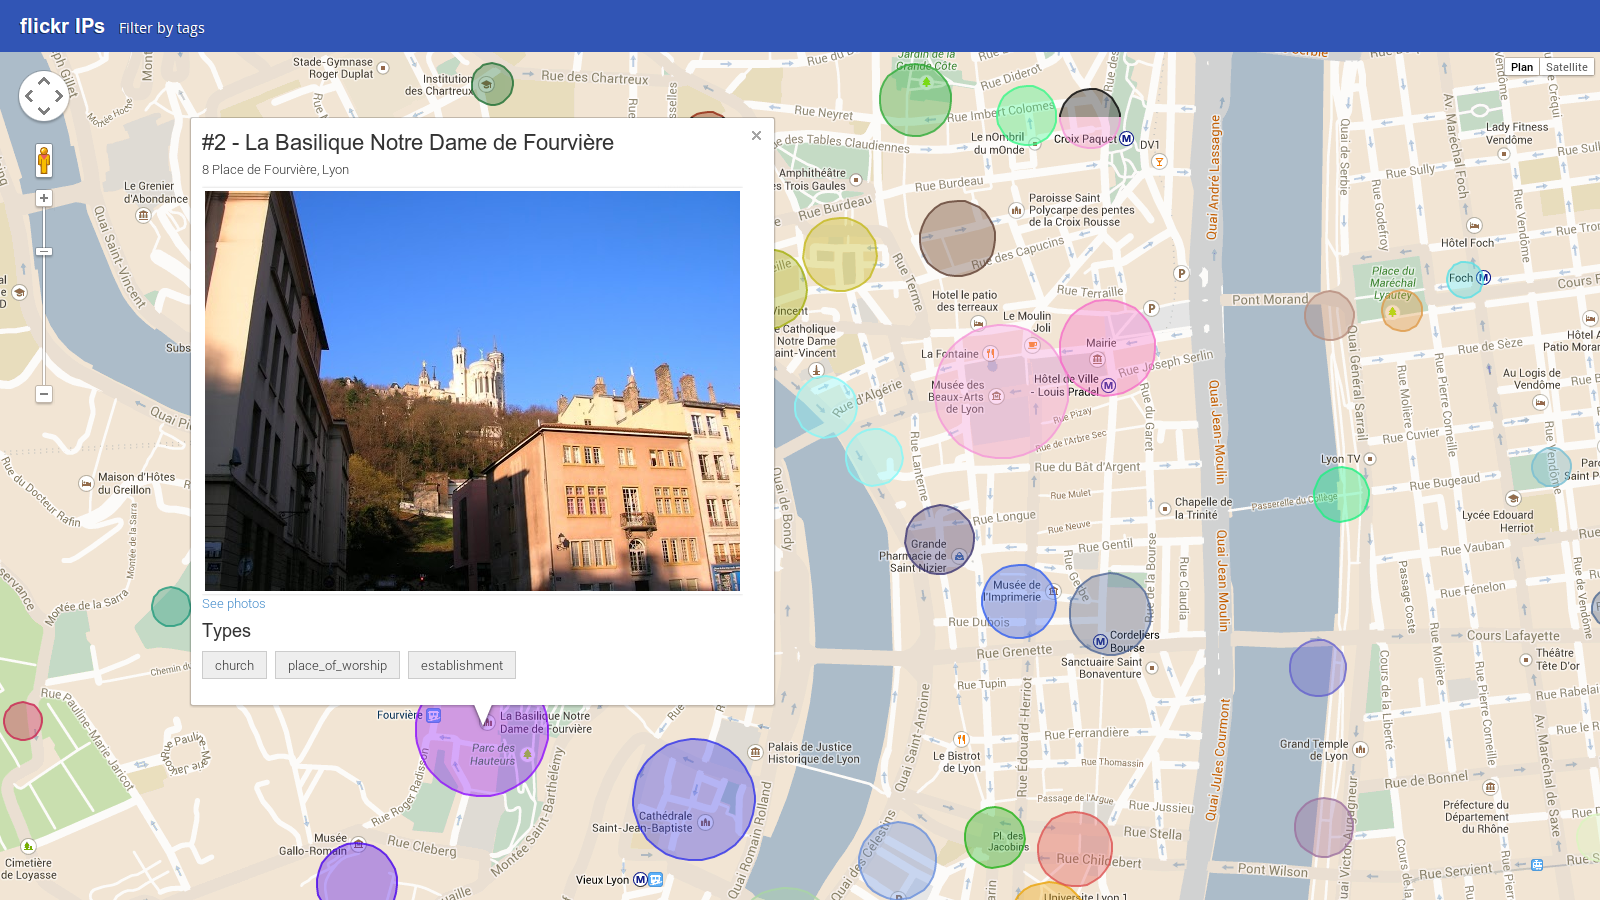
\includegraphics[scale=0.25]{../screenshots/ui-info-cluster.png}
        \caption{Informations sur un point d'intêret, ici la Basilique de Fourvière}
        \label{diagram:ui-info-cluster}
    \end{figure}

    \begin{figure}[H]
        \centering
        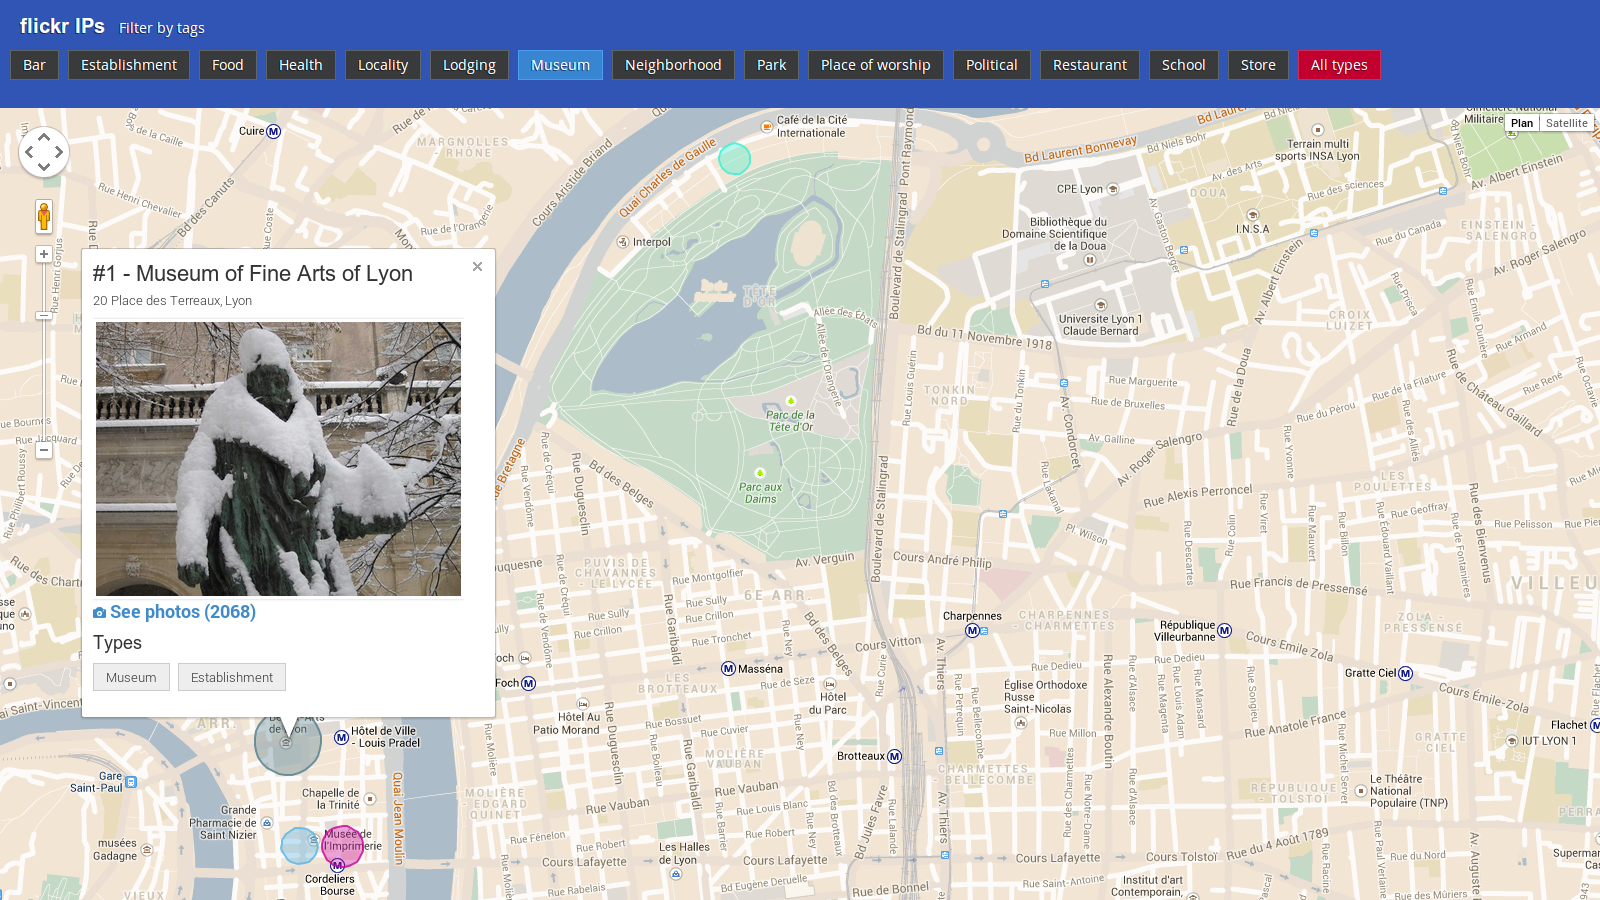
\includegraphics[scale=0.25]{../screenshots/ui-filter-museum.png}
        \caption{On peut filtrer les points d'intêret par type. Par exemple chercher un musée...}
        \label{diagram:ui-filter-museum}
    \end{figure}

    \begin{figure}[H]
        \centering
        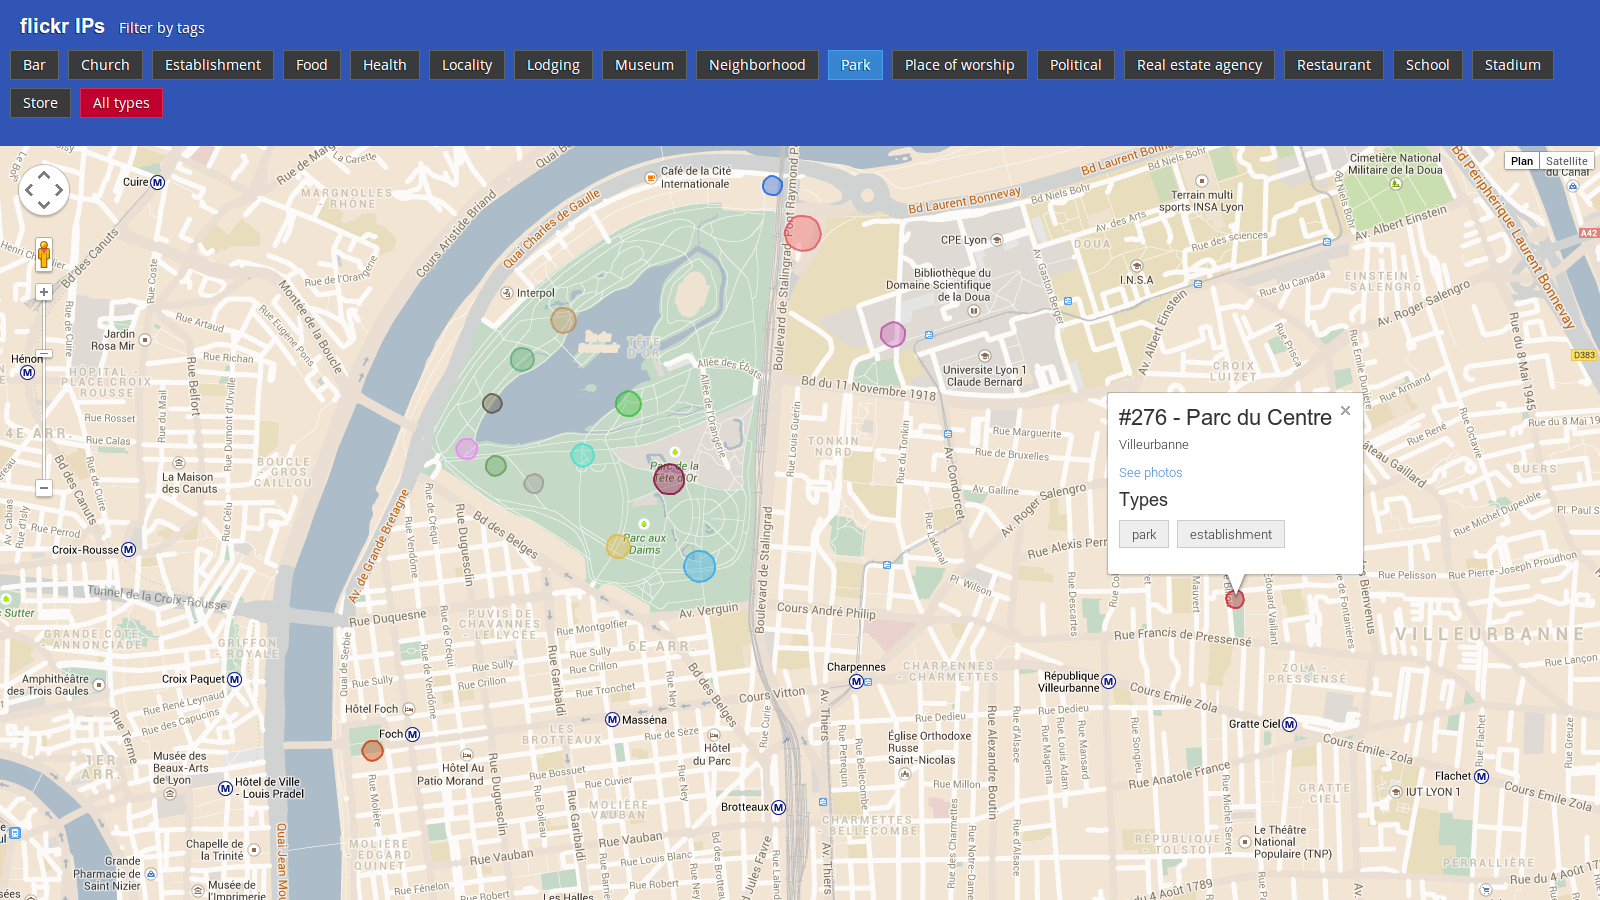
\includegraphics[scale=0.25]{../screenshots/ui-filter-park.png}
        \caption{... ou chercher un parc.}
        \label{diagram:ui-filter-park}
    \end{figure}

    \pagebreak

